\documentclass[11pt, a4paper]{article}
\usepackage{pdfpages}
\usepackage{parallel}
\usepackage[T2A]{fontenc}
\usepackage{ucs}
\usepackage[utf8x]{inputenc}
\usepackage[polish,english,russian]{babel}
\usepackage{hyperref}
\usepackage{rotating}
\usepackage[inner=2cm,top=1.8cm,outer=2cm,bottom=2.3cm,nohead]{geometry}
\usepackage{listings}
\usepackage{graphicx}
\usepackage{wrapfig}
\usepackage{longtable}
\usepackage{indentfirst}
\usepackage{array}
\usepackage{tikzsymbols}
\usepackage{soul}
\usepackage[ruled,vlined]{algorithm2e}
%\counterwithout{figure}{section} 

\usepackage{url}
\makeatletter
\g@addto@macro{\UrlBreaks}{\UrlOrds}
\makeatother

\newcolumntype{P}[1]{>{\raggedright\arraybackslash}p{#1}}
\frenchspacing
\usepackage{fixltx2e} %text sub- and superscripts
\usepackage{icomma} % коскі ў матэматычным рэжыме
\PreloadUnicodePage{4}

\newcommand{\longpage}{\enlargethispage{\baselineskip}}
\newcommand{\shortpage}{\enlargethispage{-\baselineskip}}

\def\switchlang#1{\expandafter\csname switchlang#1\endcsname}
\def\switchlangbe{
\let\saverefname=\refname%
\def\refname{Літаратура}%
\def\figurename{Іл.}%
}
\def\switchlangen{
\let\saverefname=\refname%
\def\refname{References}%
\def\figurename{Fig.}%
}
\def\switchlangru{
\let\saverefname=\refname%
\let\savefigurename=\figurename%
\def\refname{Литература}%
\def\figurename{Рис.}%
}

\hyphenation{admi-ni-stra-tive}
\hyphenation{ex-pe-ri-ence}
\hyphenation{fle-xi-bi-li-ty}
\hyphenation{Py-thon}
\hyphenation{ma-the-ma-ti-cal}
\hyphenation{re-ported}
\hyphenation{imp-le-menta-tions}
\hyphenation{pro-vides}
\hyphenation{en-gi-neering}
\hyphenation{com-pa-ti-bi-li-ty}
\hyphenation{im-pos-sible}
\hyphenation{desk-top}
\hyphenation{elec-tro-nic}
\hyphenation{com-pa-ny}
\hyphenation{de-ve-lop-ment}
\hyphenation{de-ve-loping}
\hyphenation{de-ve-lop}
\hyphenation{da-ta-ba-se}
\hyphenation{plat-forms}
\hyphenation{or-ga-ni-za-tion}
\hyphenation{pro-gramming}
\hyphenation{in-stru-ments}
\hyphenation{Li-nux}
\hyphenation{sour-ce}
\hyphenation{en-vi-ron-ment}
\hyphenation{Te-le-pathy}
\hyphenation{Li-nux-ov-ka}
\hyphenation{Open-BSD}
\hyphenation{Free-BSD}
\hyphenation{men-ti-on-ed}
\hyphenation{app-li-ca-tion}

\def\progref!#1!{\texttt{#1}}
\renewcommand{\arraystretch}{2} %Іначай формулы ў матрыцы зліпаюцца з лініямі
\usepackage{array}

\def\interview #1 (#2), #3, #4, #5\par{

\section[#1, #3, #4]{#1 -- #3, #4}
\def\qname{LVEE}
\def\aname{#1}
\def\q ##1\par{{\noindent \bf \qname: ##1 }\par}
\def\a{{\noindent \bf \aname: } \def\qname{L}\def\aname{#2}}
}

\def\interview* #1 (#2), #3, #4, #5\par{

\section*{#1\\{\small\rm #3, #4. #5}}
\ifx\ParallelWhichBox\undefined%
    \addcontentsline{toc}{section}{#1, #3, #4}%
\else%
\ifnum\ParallelWhichBox=0%
    \addcontentsline{toc}{section}{#1, #3, #4}%
\fi\fi%

\def\qname{LVEE}
\def\aname{#1}
\def\q ##1\par{{\noindent \bf \qname: ##1 }\par}
\def\a{{\noindent \bf \aname: } \def\qname{L}\def\aname{#2}}
}

\newcommand{\interviewfooter}[1]{
\vskip 1em
\noindent \textit{#1}
}

\switchlang{en}
\begin{document}

\title{1988 "--- Mouse Systems M4 PC mouse}
\date{}
\maketitle
\selectlanguage{english}
The Mouse Systems M4 mouse (fig. \ref{fig:mscM4Pic}) is a typical manipulator from the Mouse Systems company created by Stephen Kirsch in 1982 to produce the original optical mouse he invented. This model is a representative of the fourth generation (the last and record in terms of the number of copies) of Mouse Systems mice designed by Kirsch. This one is designed to work with the IBM PC serial interface, RS-232.

\begin{figure}[h]
    \centering
    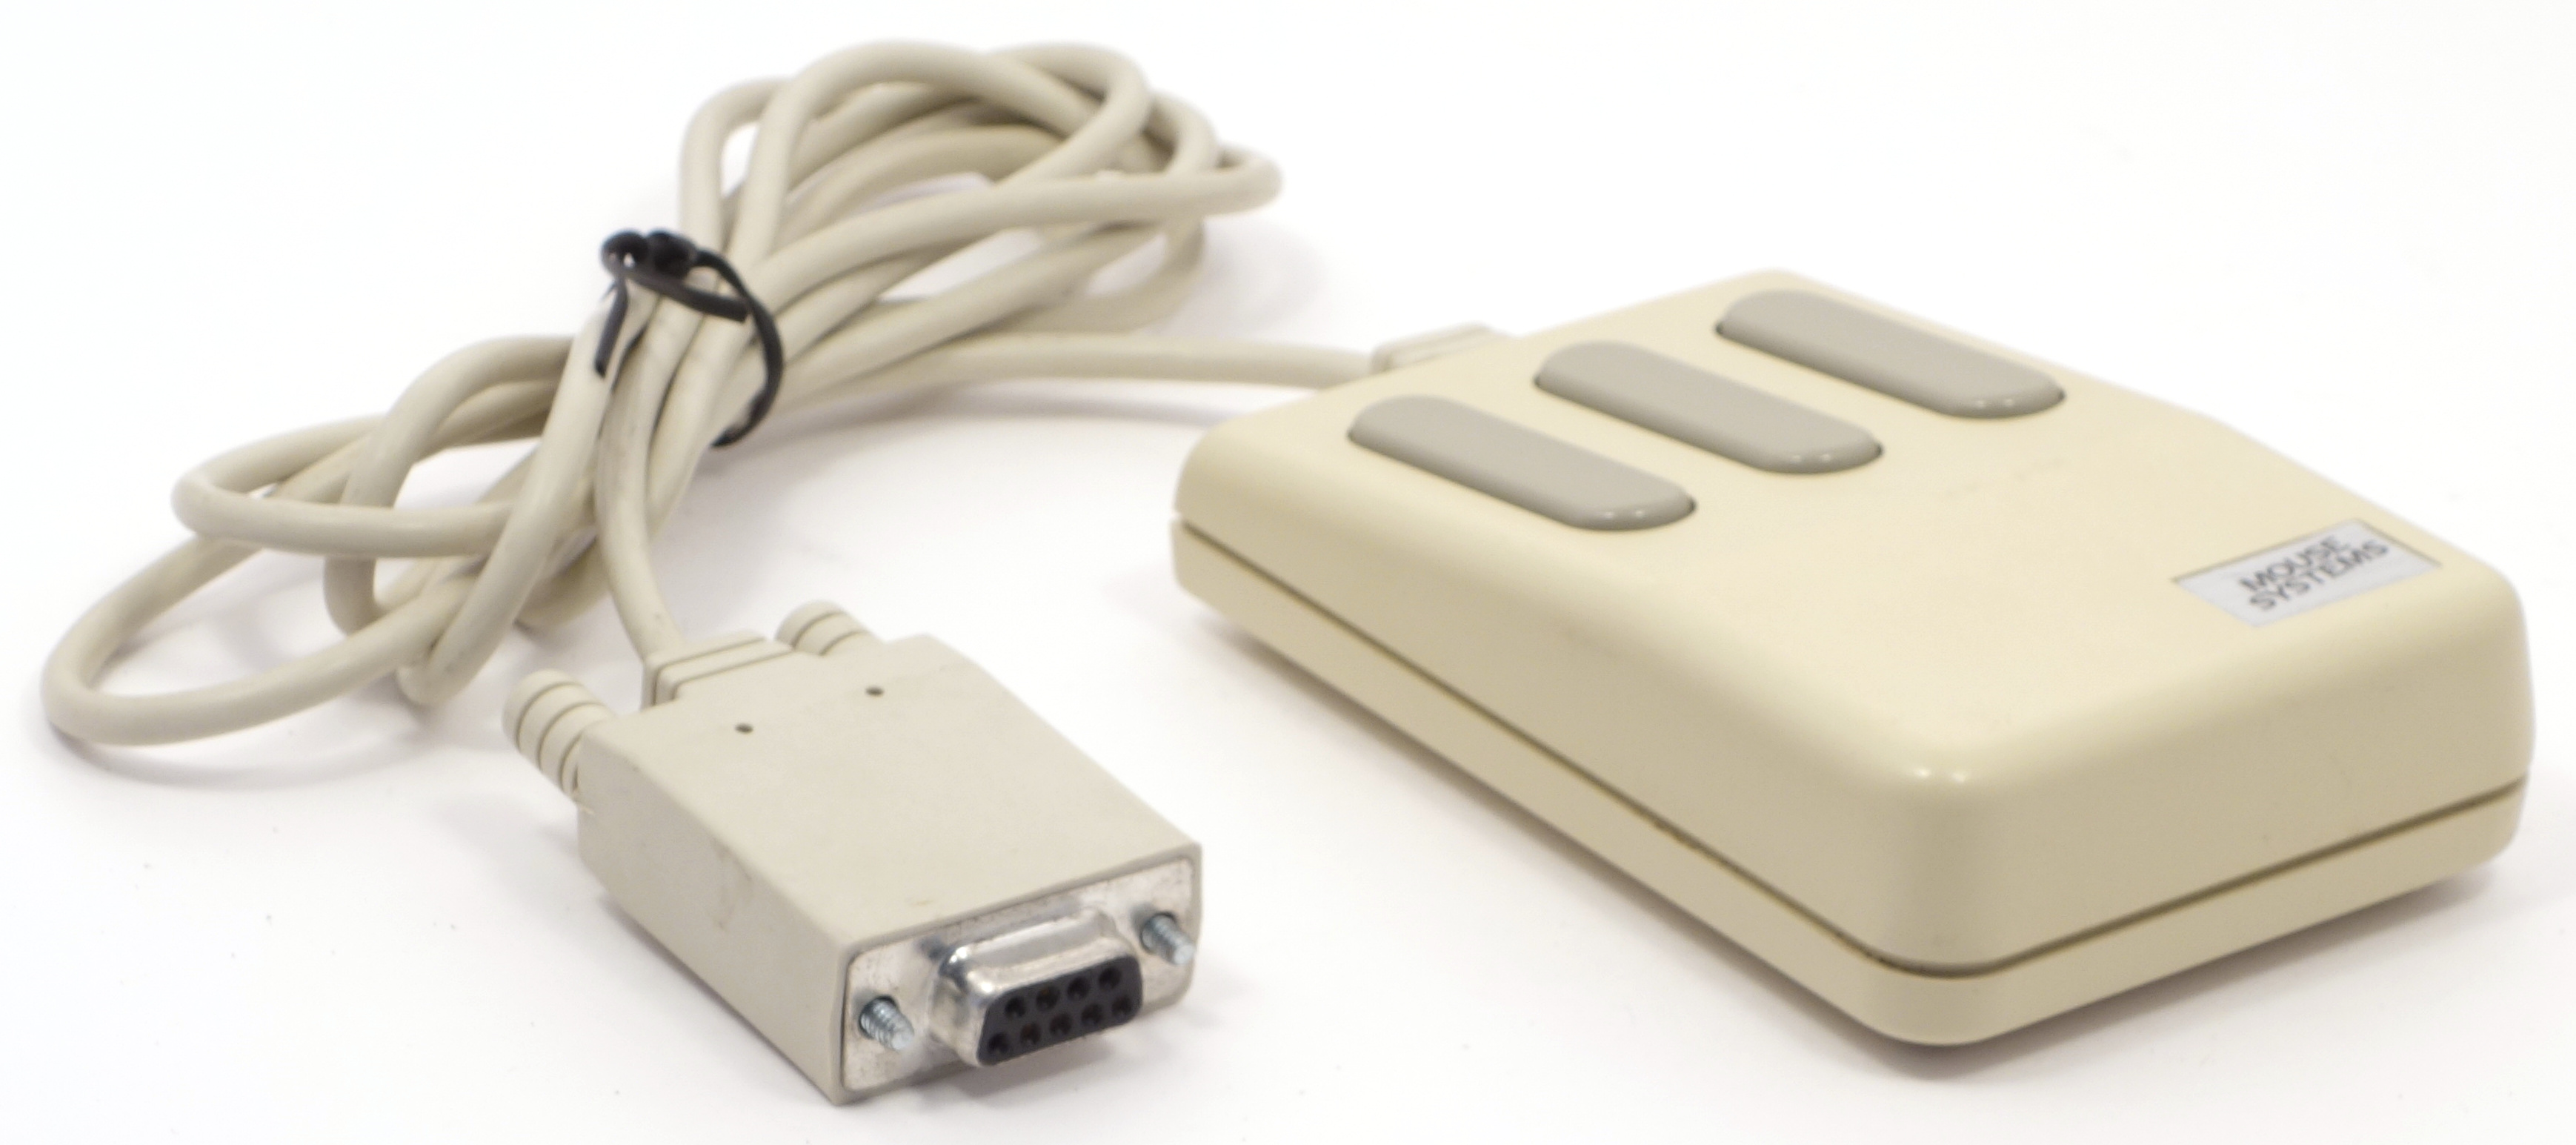
\includegraphics[scale=0.5]{1988_mouse_systems_m4/pic_30.jpg}
    \caption{Mouse Systems M4 mouse}
    \label{fig:mscM4Pic}
\end{figure}

As with all early optical mice, this mousepad requires a reflective mesh pad (fig. \ref{fig:mscM4Pad}). That is a traditional Mouse Systems metal pads with a mesh of vertical and horizontal lines for two different wavelengths (for the optical and infrared ranges).

\begin{figure}[h]
    \centering
    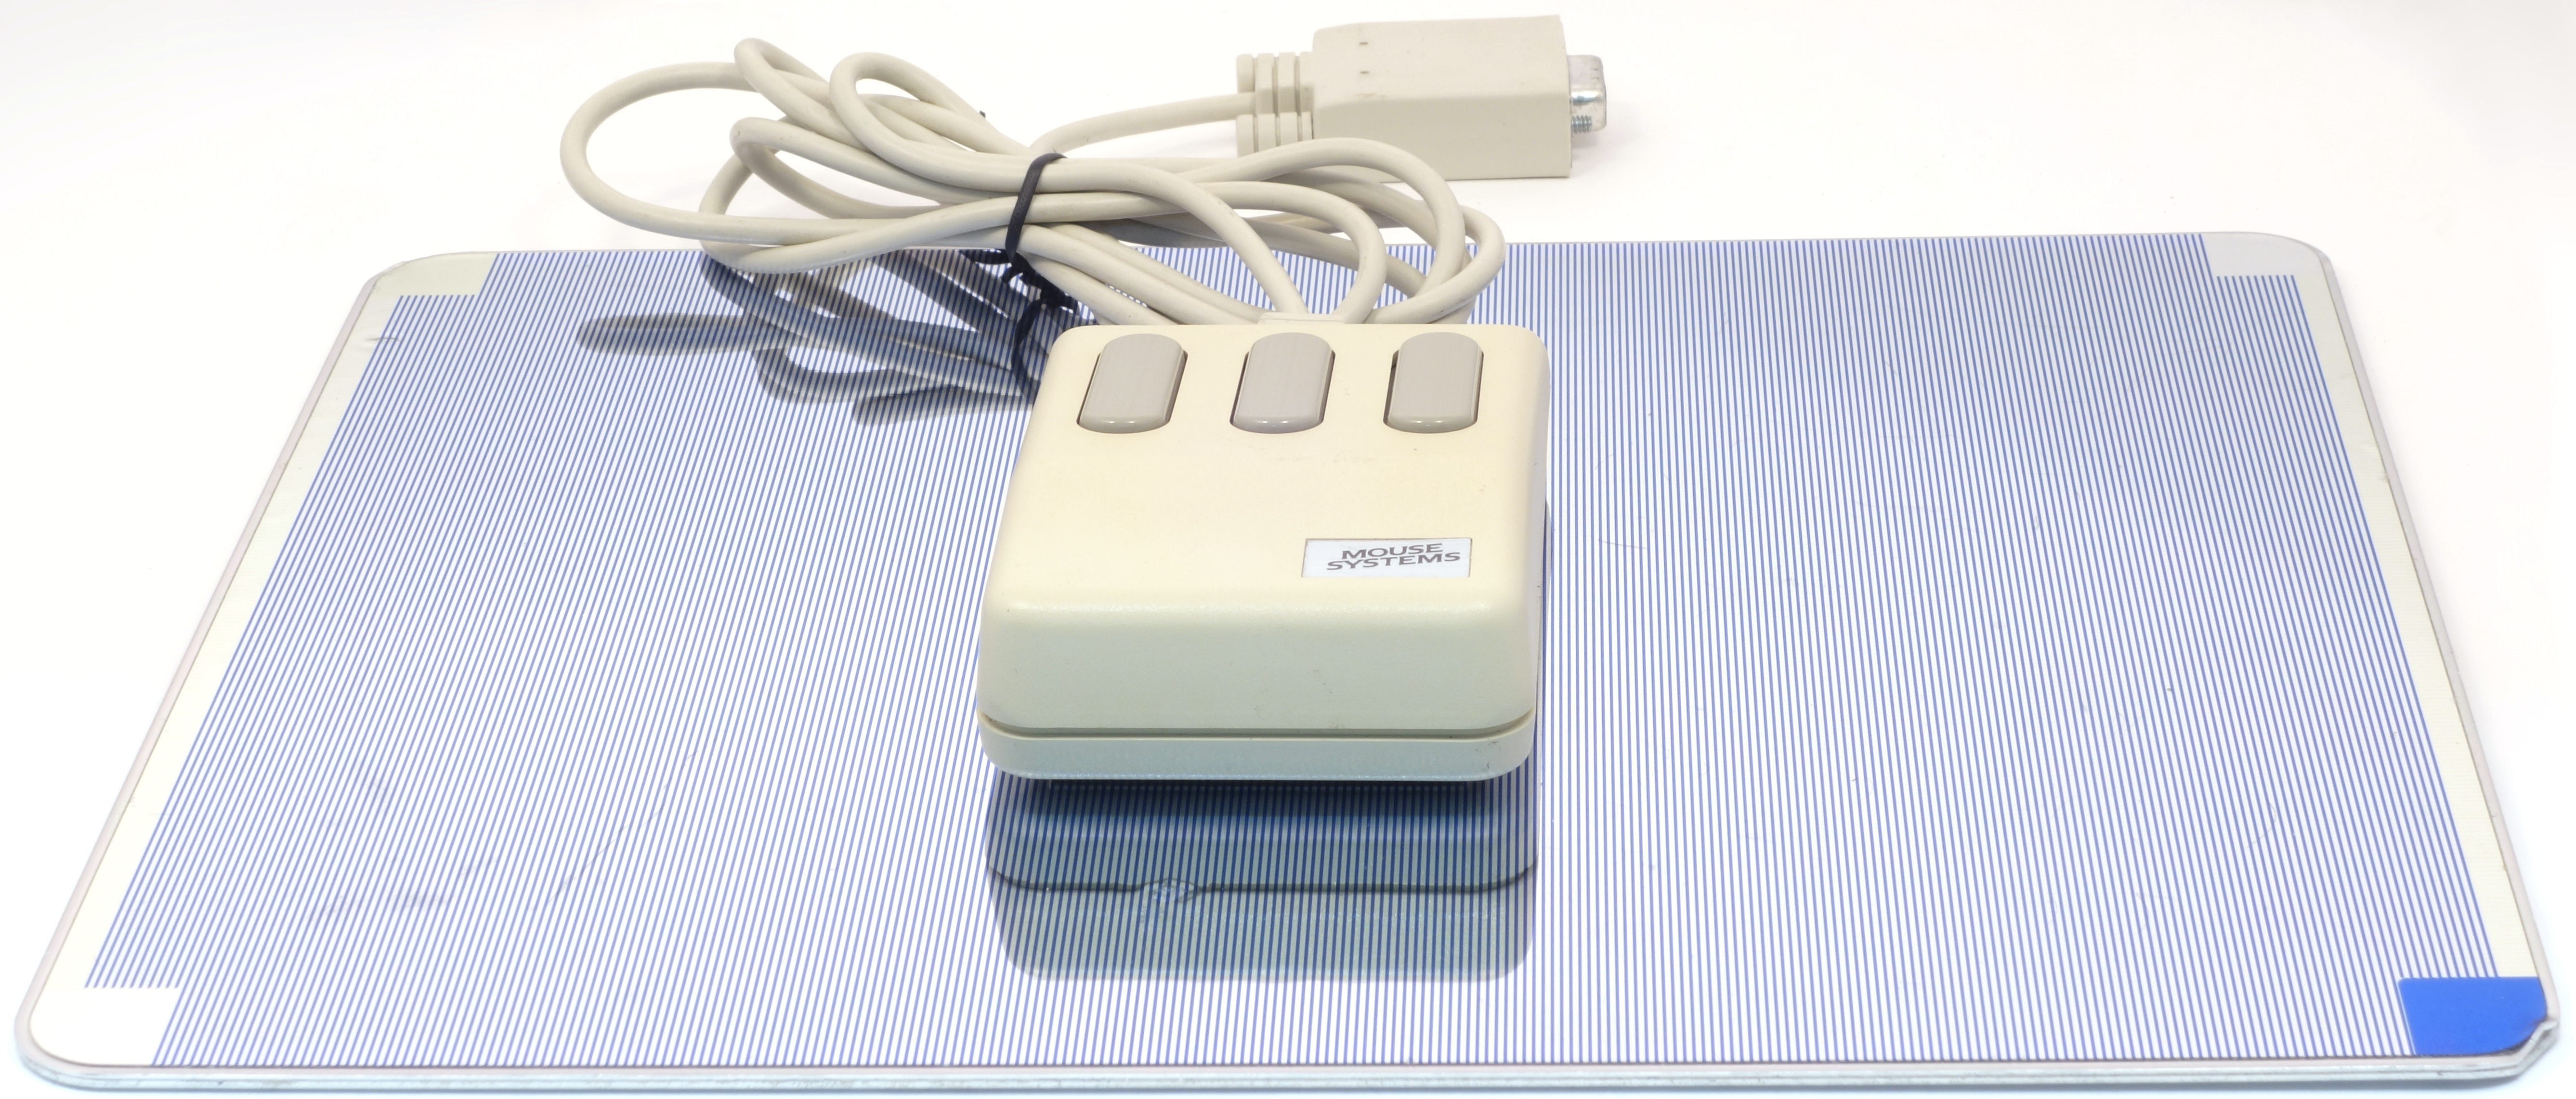
\includegraphics[scale=0.4]{1988_mouse_systems_m4/pad_30.jpg}
    \caption{Mouse Systems M4 mouse on its pad}
    \label{fig:mscM4Pad}
\end{figure}

The mouse is made in a standard case for Mouse Systems -- a flat rectangle with three elongated rounded buttons. On the upper side of the case there is a plate with the name of the company, typed in capital italics, on the lower side -- the same name and an emblem in the form of two triangles stylized as an image of a mouse and a screen cursor (fig. \ref{fig:mscM4TopBottom}). Unlike earlier Mouse Systems mice with an RS-232 interface (such as the M2 mouse), the M4 uses less power-hungry LEDs and therefore does not require an additional power supply.

The FCC ID code reveals that this mouse was presented by Mouse Systems in 1988.

\begin{figure}[h]
    \centering
    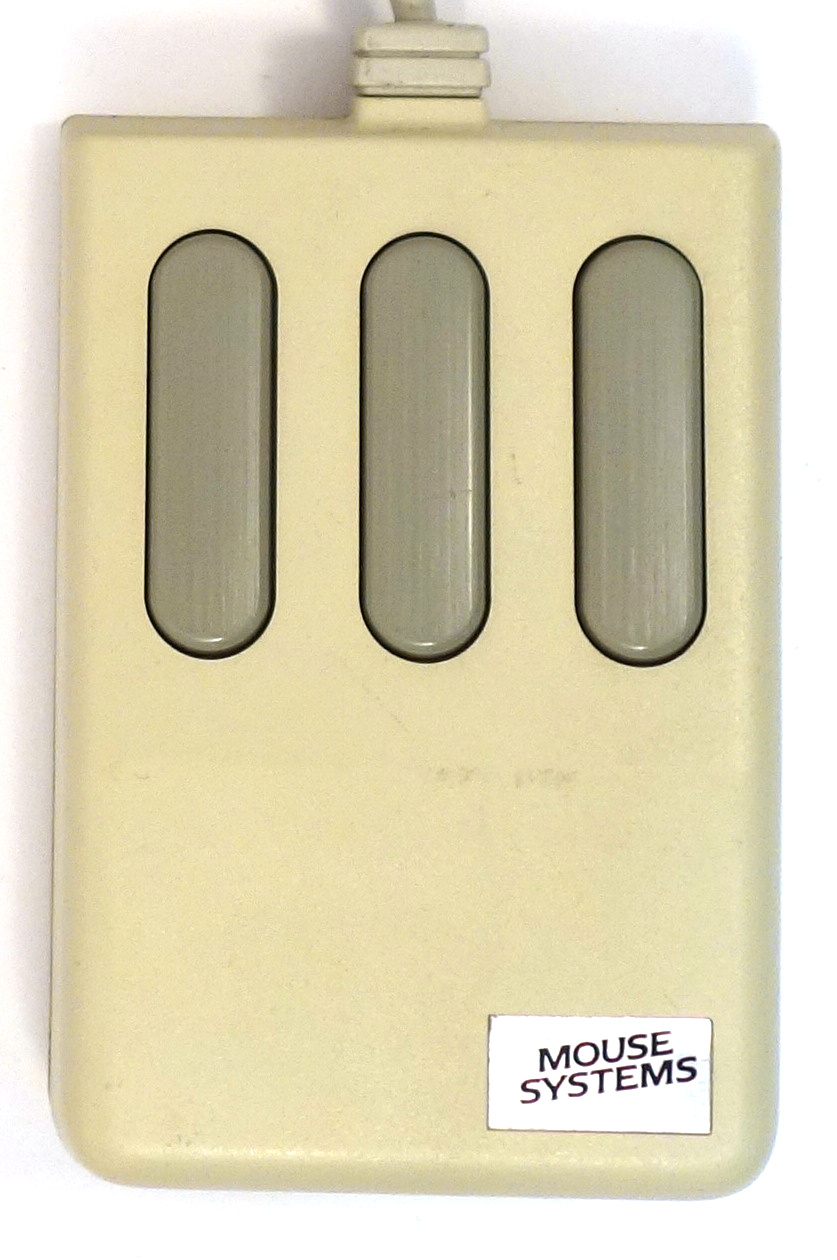
\includegraphics[scale=0.7]{1988_mouse_systems_m4/top_30.jpg}
    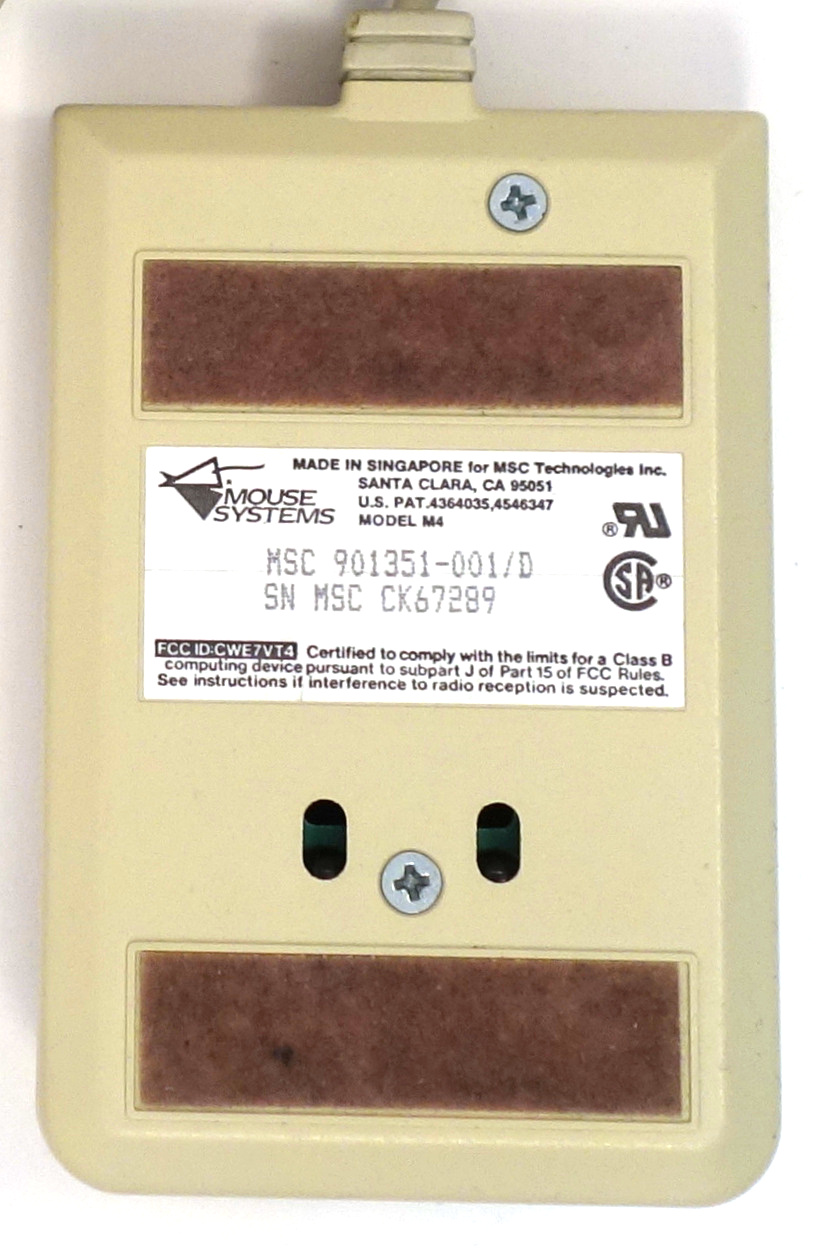
\includegraphics[scale=0.7]{1988_mouse_systems_m4/bottom_30.jpg}
    \caption{Mouse Systems M4 mouse, top and bottom views}
    \label{fig:mscM4TopBottom}
\end{figure}

The small flat case (fig. \ref{fig:mscM4Size}) clearly illustrates the absence of the ball and other mechanical elements \cite{pcmag}; it has been quite successful and has not changed in size and shape since the first generation \cite{old} mice.

\begin{figure}[h]
    \centering
    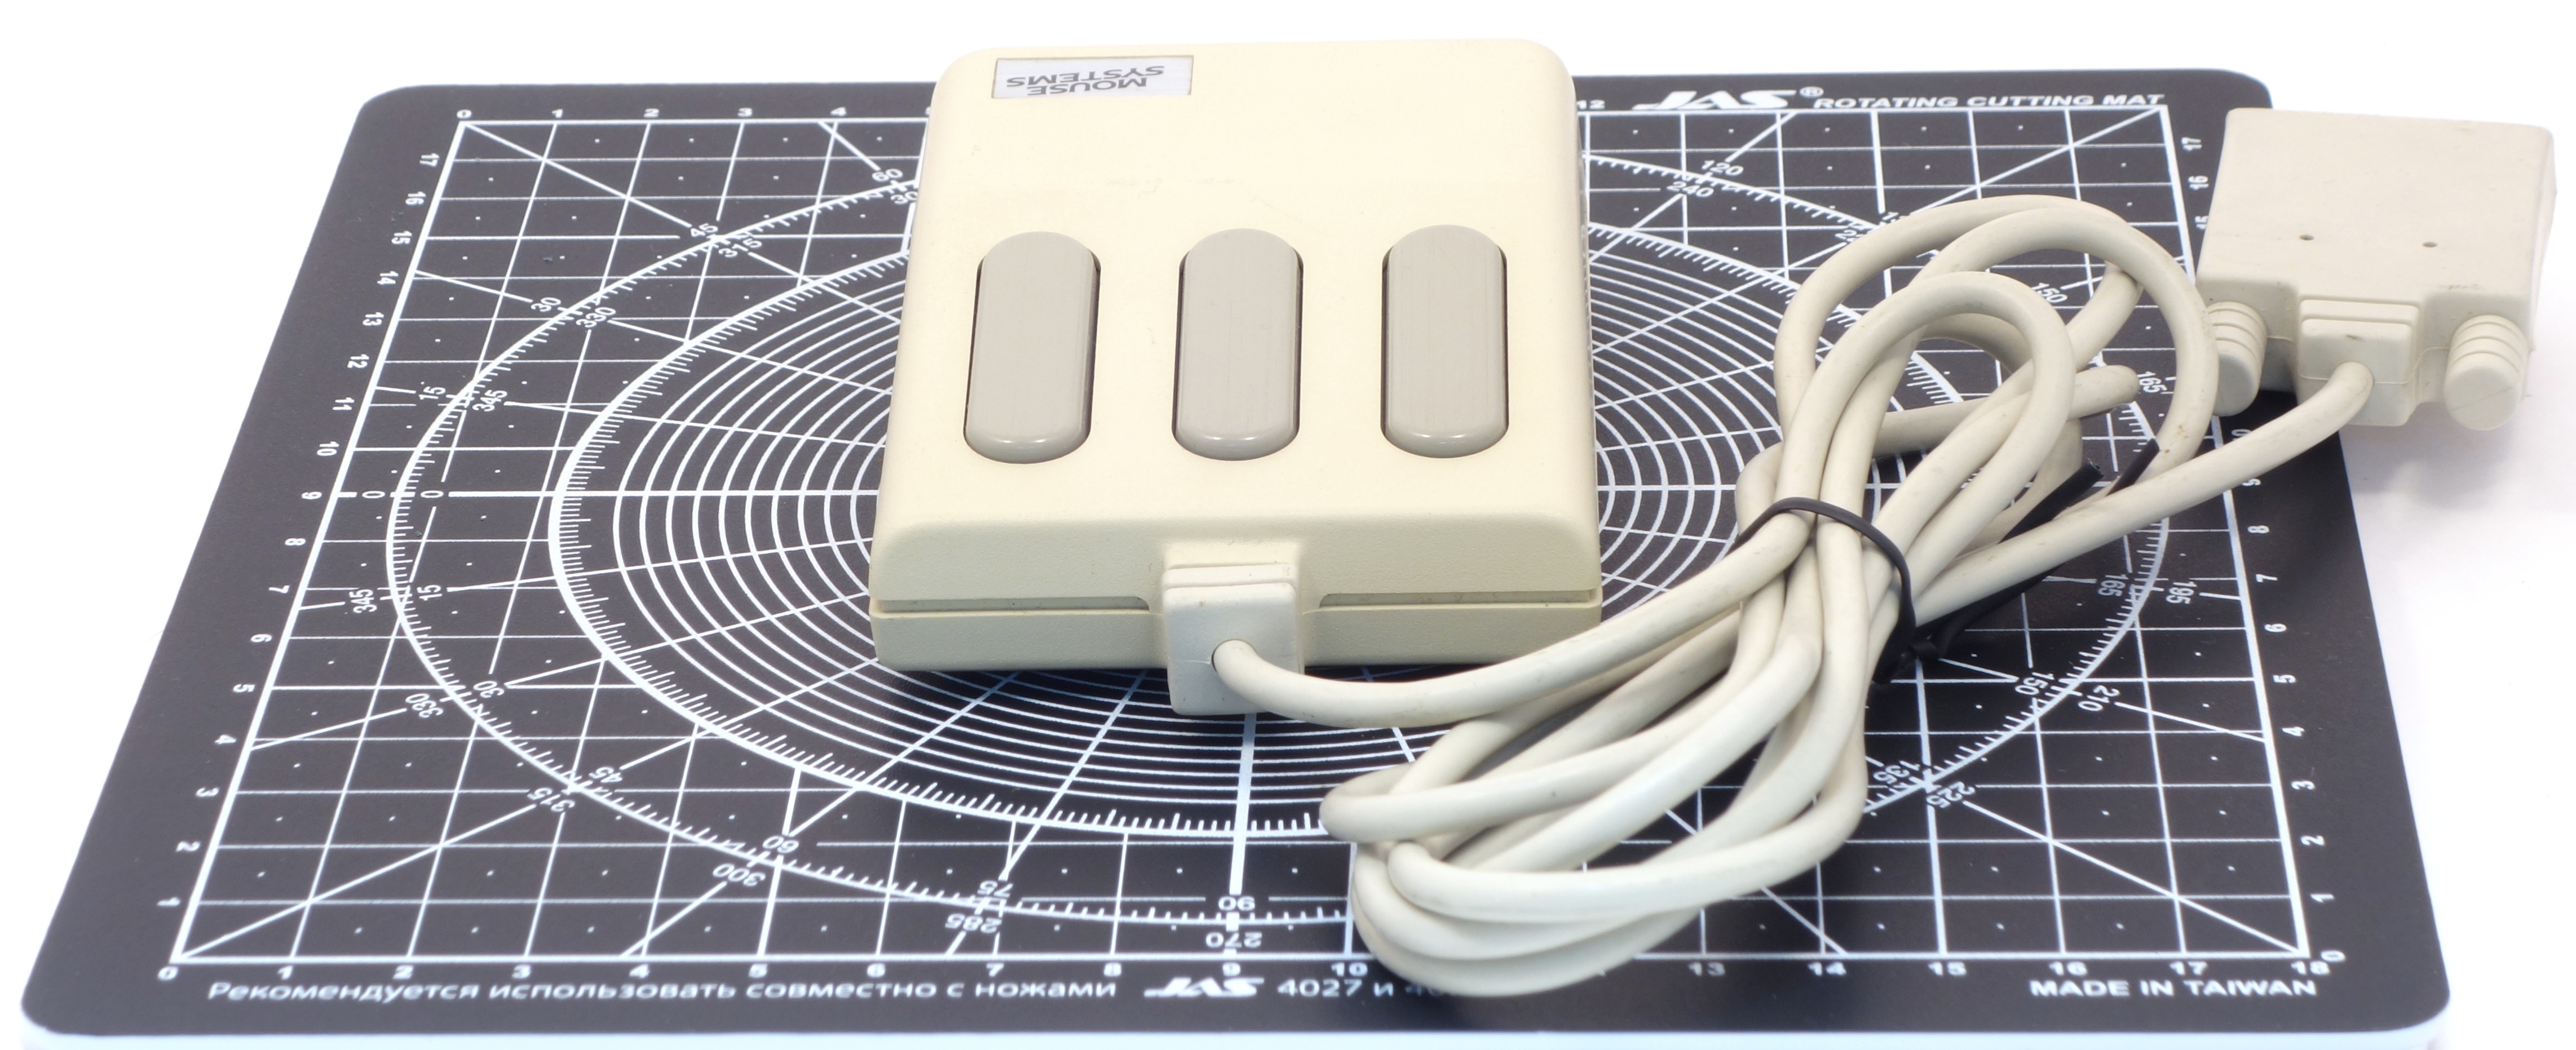
\includegraphics[width=\textwidth]{1988_mouse_systems_m4/size_30.jpg}
    \caption{Mouse Systems M4 mouse on a graduated pad with a grid step of 1~cm}
    \label{fig:mscM4Size}
\end{figure}

The mouse has a fairly ergonomic shape by the standards of the 80s (Fig. \ref{fig:mscM4Hand}) thanks to a rather successful shape with rounded corners and large buttons. The lack of wrist support is less noticeable due to the low body height of the mouse, and the buttons are among the most ergonomic ones of the 80s mice.

\begin{figure}[h]
    \centering
    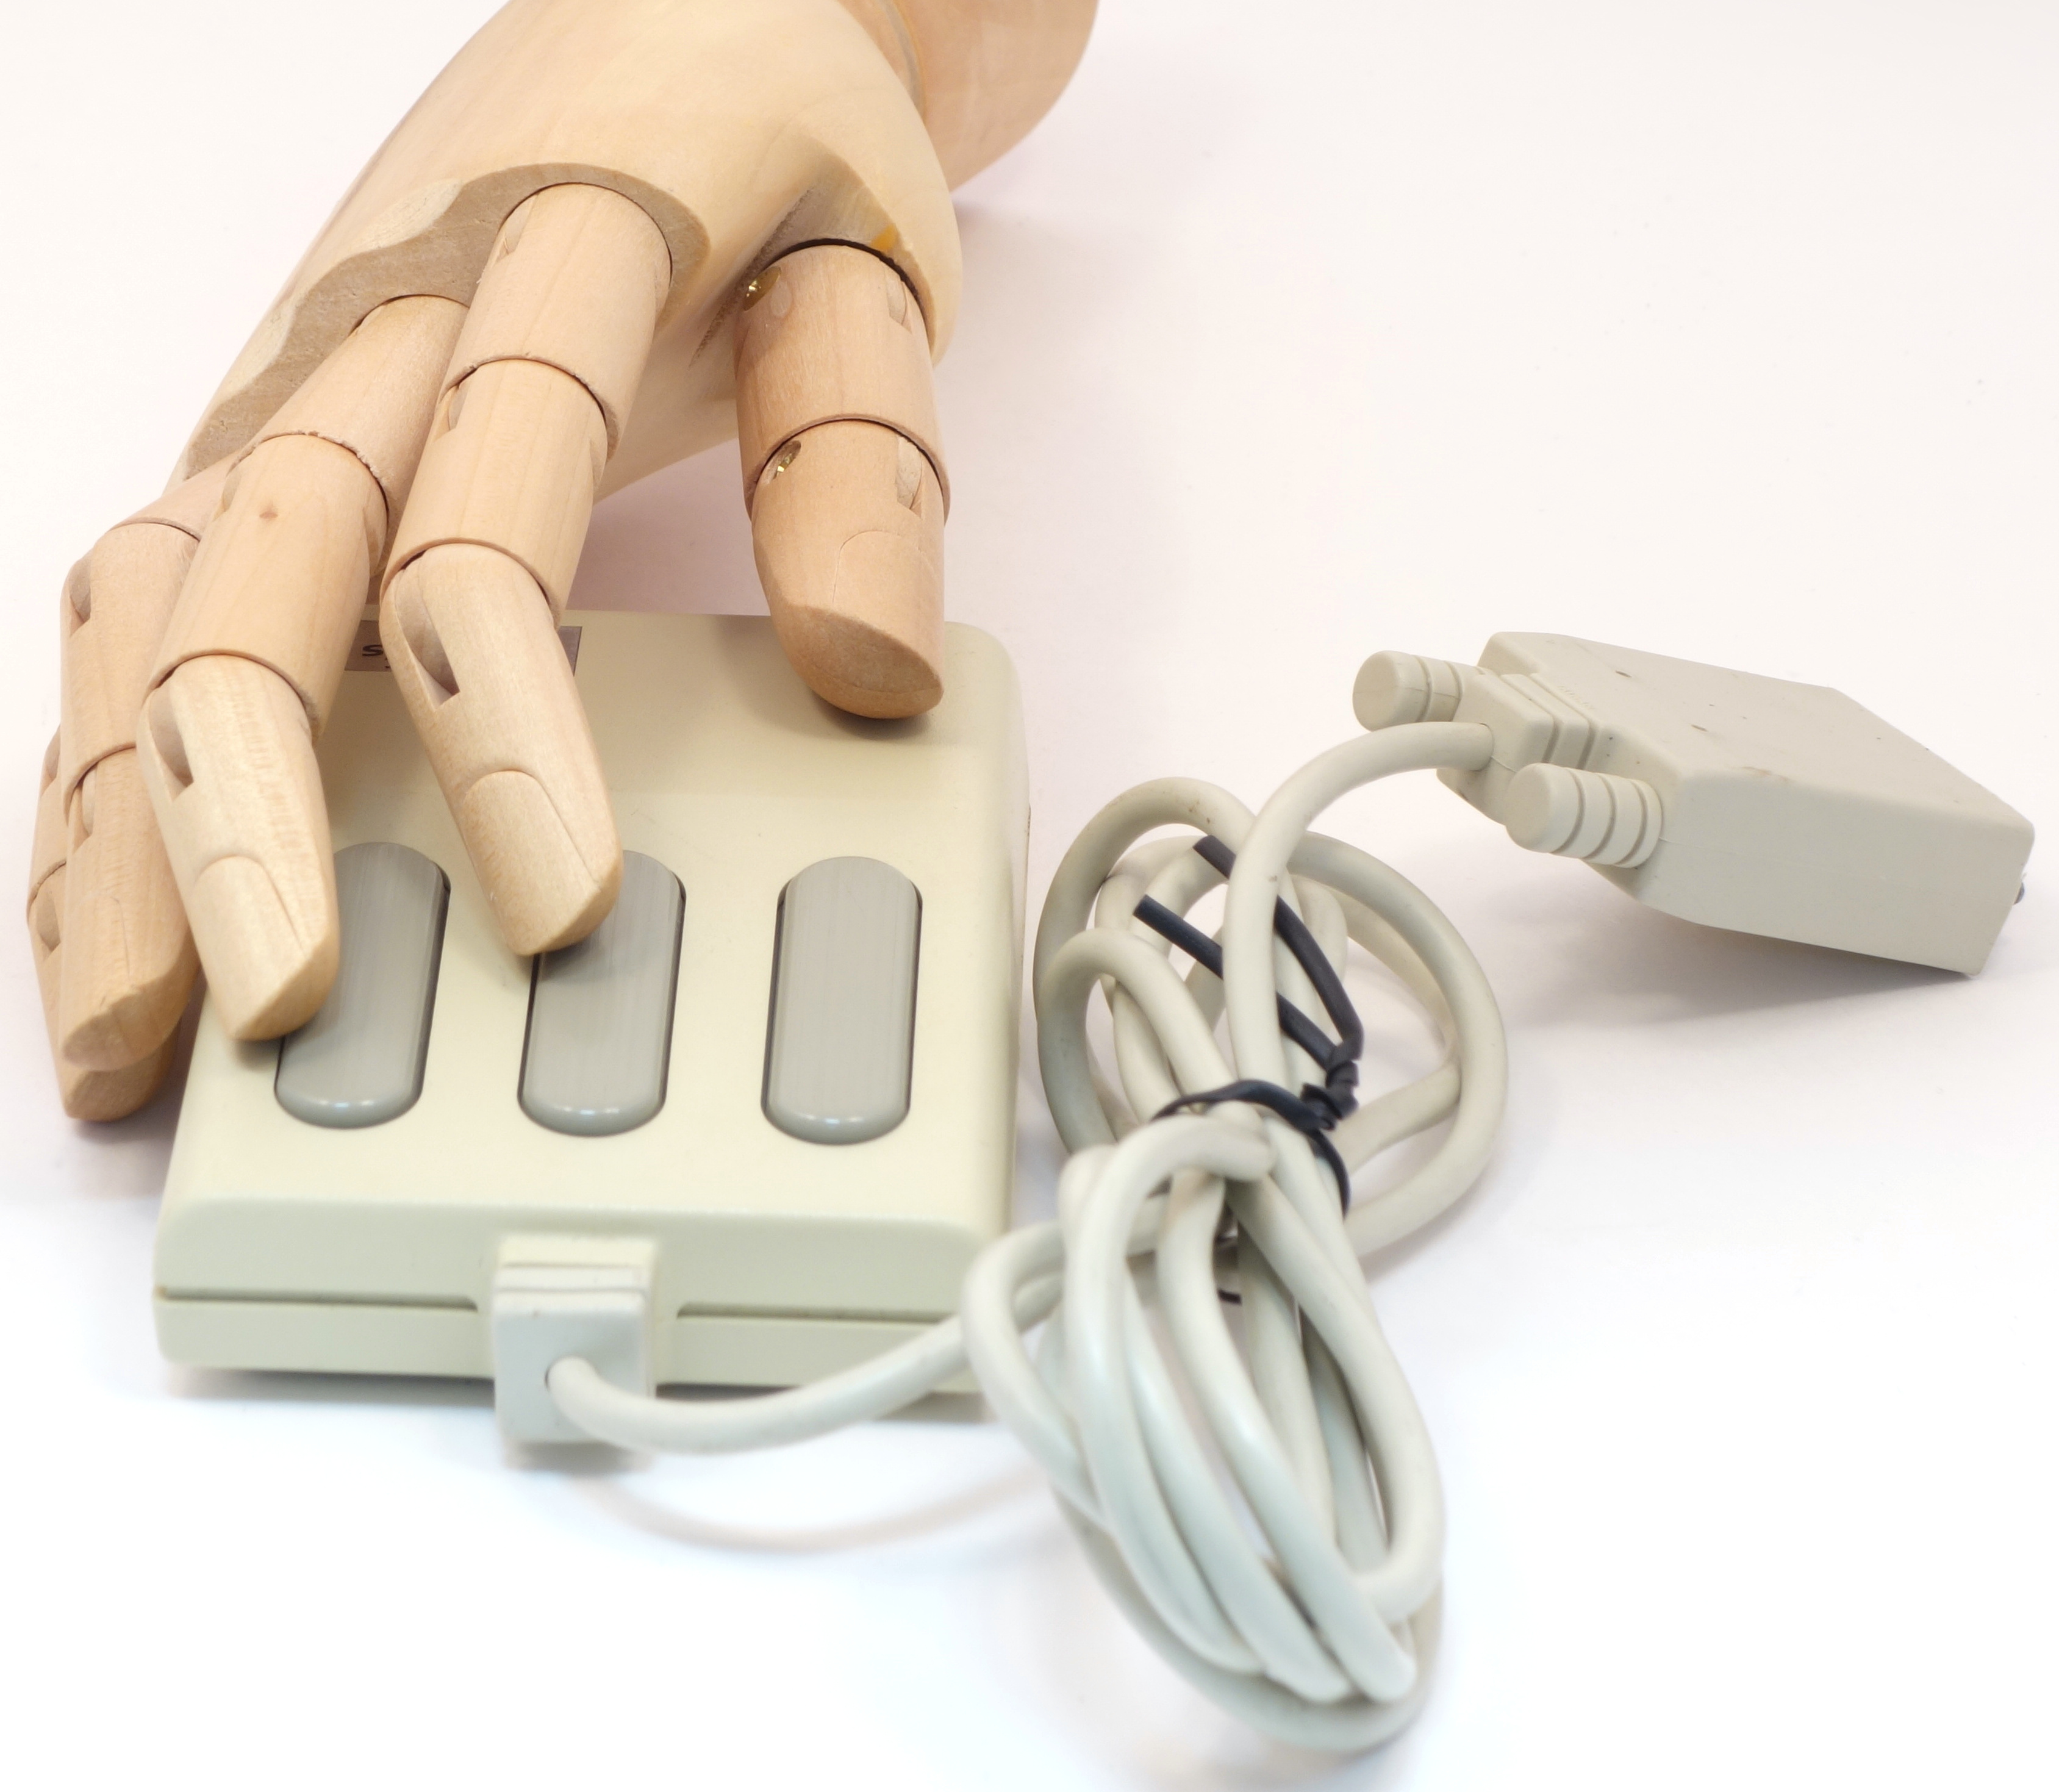
\includegraphics[scale=0.35]{1988_mouse_systems_m4/hand_30.jpg}
    \caption{Mouse Systems M4 with a human hand model}
    \label{fig:mscM4Hand}
\end{figure}

The internals are shown in fig. \ref{fig:mscM4Inside}.

In accordance with the scheme invented by Kirsch, the light emitted by the LEDs is reflected from the pad, then from the lustrous foil plate in the upper part of the mouse body, and finally falls on two lines of photodetectors, one of which is located along the longitudinal axis, and the other along the transverse one. One of the LEDs emits light in the optical range, in which the transverse lines printed on the pad are visible, and the other emits infrared light, in which the longitudinal lines are visible. When the mouse moves, the alternation of lines is read by the corresponding line of photodetectors. Fig. \ref{fig:mscM4Inside} shows two lines of photodetectors (4 in each): this is an improved design compared to the original version by Steve Kirsch (first generation of Mouse Systems mice used a single photodetector matrix of $2 \times 2$, the disadvantage of which was the mouse calibration period after each power-up, during which the microcontroller performed automatic selection of the correct threshold values for the photodetectors) \cite{bio}.

\begin{figure}[h]
    \centering
    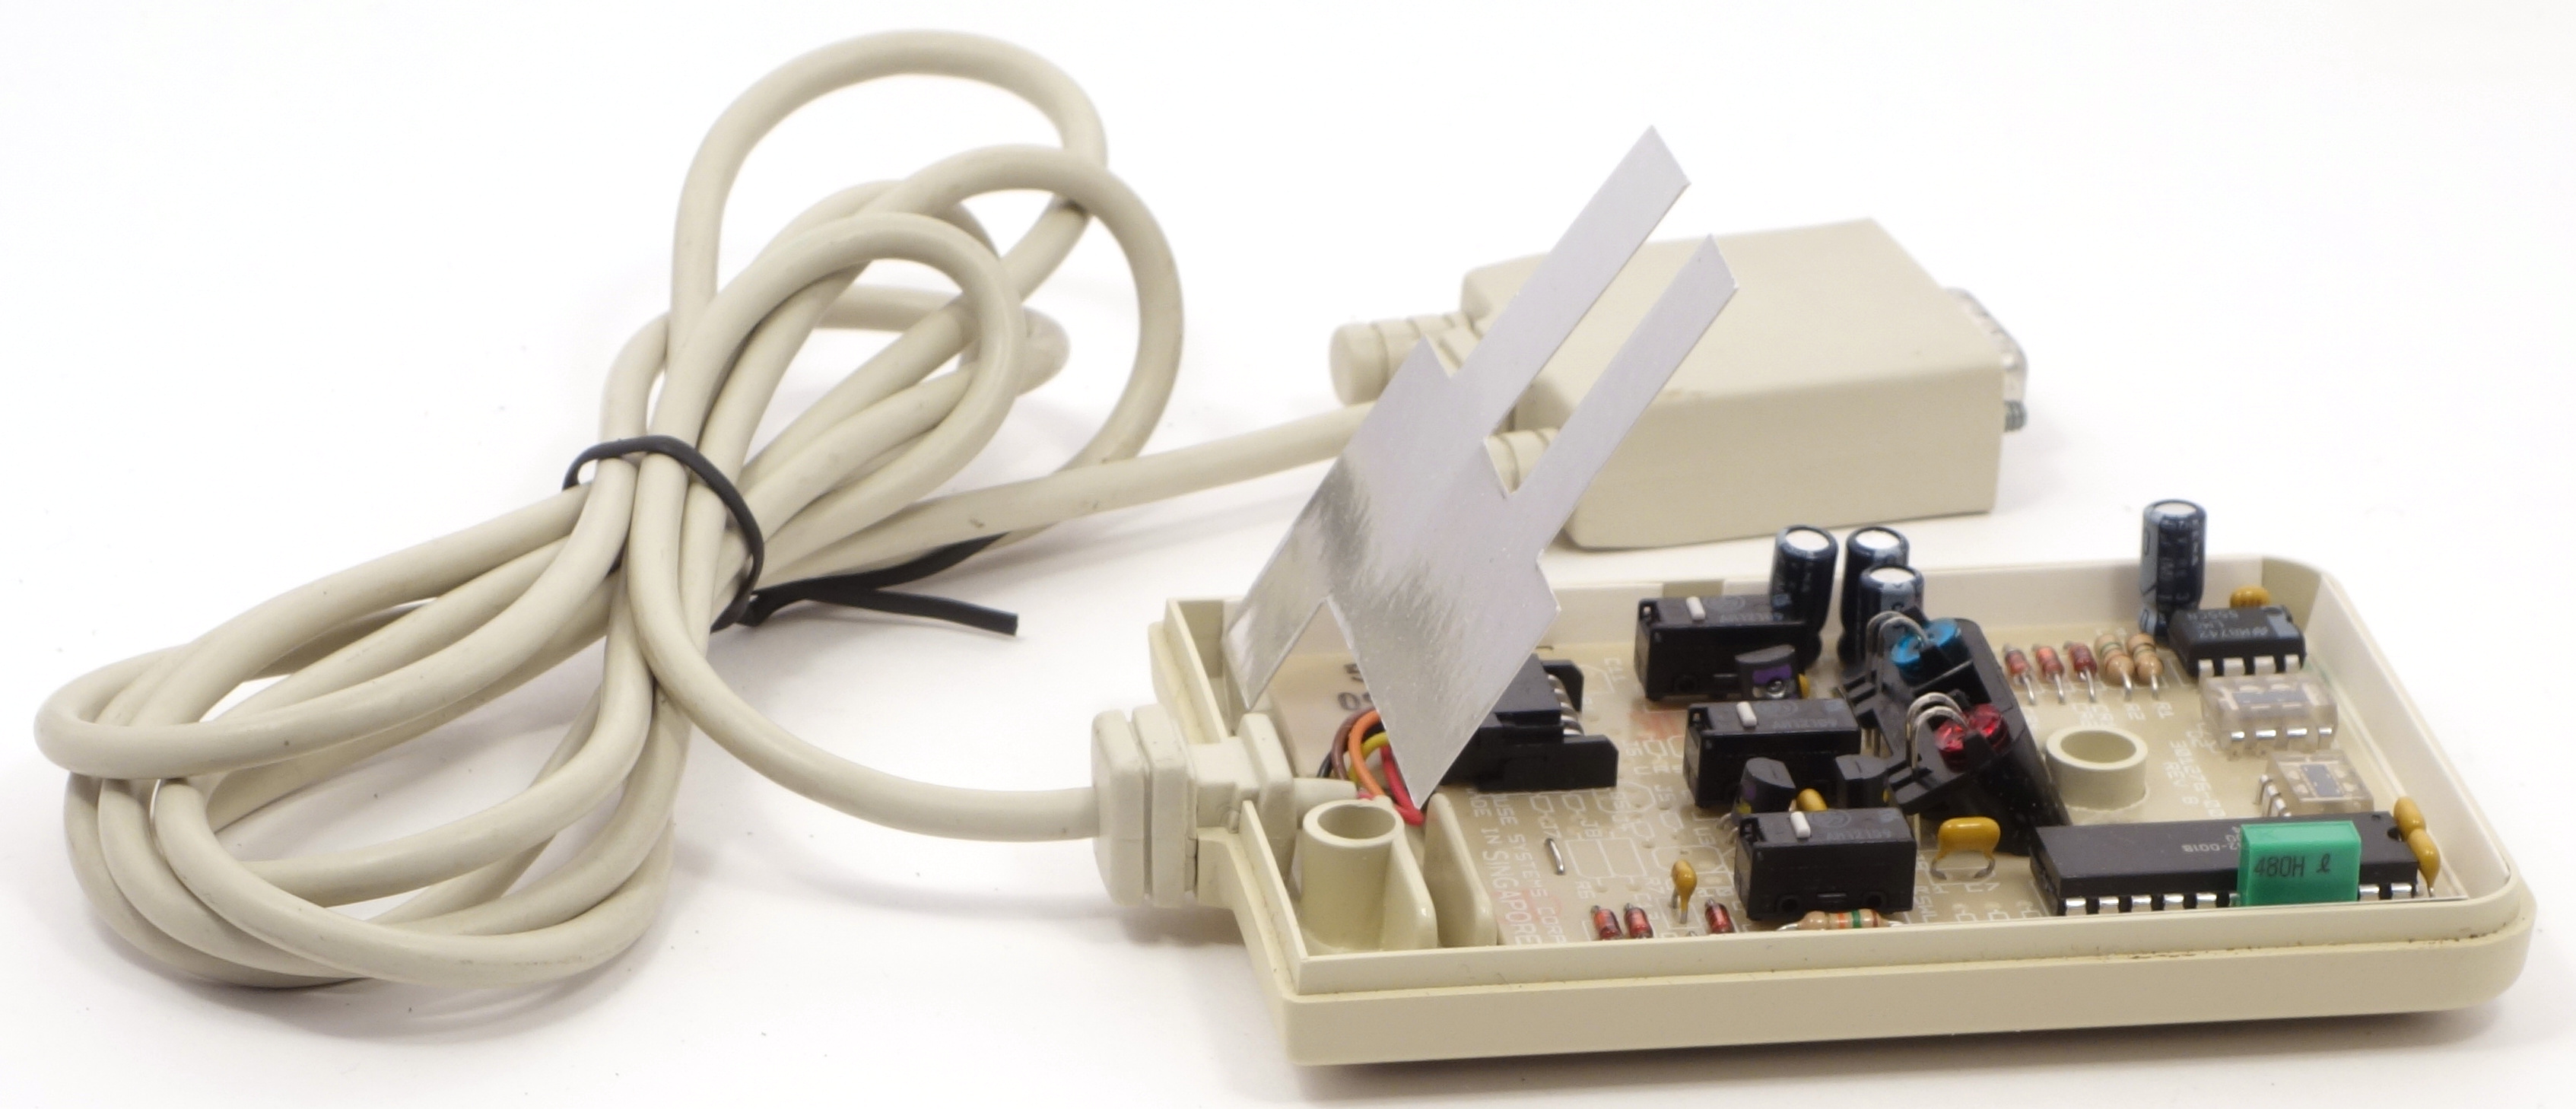
\includegraphics[scale=0.6]{1988_mouse_systems_m4/inside_30.jpg}
    \caption{Mouse Systems M4 mouse disassembled}
    \label{fig:mscM4Inside}
\end{figure}

\begin{thebibliography}{9}
\bibitem {pcmag} Why you should buy the mouse with no moving parts [adv.] // PC MAGAZINE, V. 7, No. 3, February 16, 1988. P. 205. \url{https://archive.org/details/PC-Mag-1988-02-16/page/n203/mode/2up}
\bibitem {old} Mouse Systems -- oldmouse.com  \url{https://web.archive.org/web/20211205082304/http://oldmouse.com/mouse/mousesystems/}
\bibitem {bio} Perry S.T. Steve Kirsch -- IEEE Spectrum. 01 AUG 2000 \url{https://spectrum.ieee.org/steve-kirsch}
\end{thebibliography}
\end{document}
